\documentclass[1p]{elsarticle_modified}
%\bibliographystyle{elsarticle-num}

%\usepackage[colorlinks]{hyperref}
%\usepackage{abbrmath_seonhwa} %\Abb, \Ascr, \Acal ,\Abf, \Afrak
\usepackage{amsfonts}
\usepackage{amssymb}
\usepackage{amsmath}
\usepackage{amsthm}
\usepackage{scalefnt}
\usepackage{amsbsy}
\usepackage{kotex}
\usepackage{caption}
\usepackage{subfig}
\usepackage{color}
\usepackage{graphicx}
\usepackage{xcolor} %% white, black, red, green, blue, cyan, magenta, yellow
\usepackage{float}
\usepackage{setspace}
\usepackage{hyperref}

\usepackage{tikz}
\usetikzlibrary{arrows}

\usepackage{multirow}
\usepackage{array} % fixed length table
\usepackage{hhline}

%%%%%%%%%%%%%%%%%%%%%
\makeatletter
\renewcommand*\env@matrix[1][\arraystretch]{%
	\edef\arraystretch{#1}%
	\hskip -\arraycolsep
	\let\@ifnextchar\new@ifnextchar
	\array{*\c@MaxMatrixCols c}}
\makeatother %https://tex.stackexchange.com/questions/14071/how-can-i-increase-the-line-spacing-in-a-matrix
%%%%%%%%%%%%%%%

\usepackage[normalem]{ulem}

\newcommand{\msout}[1]{\ifmmode\text{\sout{\ensuremath{#1}}}\else\sout{#1}\fi}
%SOURCE: \msout is \stkout macro in https://tex.stackexchange.com/questions/20609/strikeout-in-math-mode

\newcommand{\cancel}[1]{
	\ifmmode
	{\color{red}\msout{#1}}
	\else
	{\color{red}\sout{#1}}
	\fi
}

\newcommand{\add}[1]{
	{\color{blue}\uwave{#1}}
}

\newcommand{\replace}[2]{
	\ifmmode
	{\color{red}\msout{#1}}{\color{blue}\uwave{#2}}
	\else
	{\color{red}\sout{#1}}{\color{blue}\uwave{#2}}
	\fi
}

\newcommand{\Sol}{\mathcal{S}} %segment
\newcommand{\D}{D} %diagram
\newcommand{\A}{\mathcal{A}} %arc


%%%%%%%%%%%%%%%%%%%%%%%%%%%%%5 test

\def\sl{\operatorname{\textup{SL}}(2,\Cbb)}
\def\psl{\operatorname{\textup{PSL}}(2,\Cbb)}
\def\quan{\mkern 1mu \triangleright \mkern 1mu}

\theoremstyle{definition}
\newtheorem{thm}{Theorem}[section]
\newtheorem{prop}[thm]{Proposition}
\newtheorem{lem}[thm]{Lemma}
\newtheorem{ques}[thm]{Question}
\newtheorem{cor}[thm]{Corollary}
\newtheorem{defn}[thm]{Definition}
\newtheorem{exam}[thm]{Example}
\newtheorem{rmk}[thm]{Remark}
\newtheorem{alg}[thm]{Algorithm}

\newcommand{\I}{\sqrt{-1}}
\begin{document}

%\begin{frontmatter}
%
%\title{Boundary parabolic representations of knots up to 8 crossings}
%
%%% Group authors per affiliation:
%\author{Yunhi Cho} 
%\address{Department of Mathematics, University of Seoul, Seoul, Korea}
%\ead{yhcho@uos.ac.kr}
%
%
%\author{Seonhwa Kim} %\fnref{s_kim}}
%\address{Center for Geometry and Physics, Institute for Basic Science, Pohang, 37673, Korea}
%\ead{ryeona17@ibs.re.kr}
%
%\author{Hyuk Kim}
%\address{Department of Mathematical Sciences, Seoul National University, Seoul 08826, Korea}
%\ead{hyukkim@snu.ac.kr}
%
%\author{Seokbeom Yoon}
%\address{Department of Mathematical Sciences, Seoul National University, Seoul, 08826,  Korea}
%\ead{sbyoon15@snu.ac.kr}
%
%\begin{abstract}
%We find all boundary parabolic representation of knots up to 8 crossings.
%
%\end{abstract}
%\begin{keyword}
%    \MSC[2010] 57M25 
%\end{keyword}
%
%\end{frontmatter}

%\linenumbers
%\tableofcontents
%
\newcommand\colored[1]{\textcolor{white}{\rule[-0.35ex]{0.8em}{1.4ex}}\kern-0.8em\color{red} #1}%
%\newcommand\colored[1]{\textcolor{white}{ #1}\kern-2.17ex	\textcolor{white}{ #1}\kern-1.81ex	\textcolor{white}{ #1}\kern-2.15ex\color{red}#1	}

{\Large $\underline{12a_{0318}~(K12a_{0318})}$}

\setlength{\tabcolsep}{10pt}
\renewcommand{\arraystretch}{1.6}
\vspace{1cm}\begin{tabular}{m{100pt}>{\centering\arraybackslash}m{274pt}}
\multirow{5}{120pt}{
	\centering
	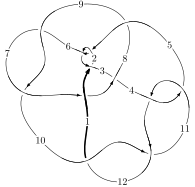
\includegraphics[width=112pt]{../../../GIT/diagram.site/Diagrams/png/1119_12a_0318.png}\\
\ \ \ A knot diagram\footnotemark}&
\allowdisplaybreaks
\textbf{Linearized knot diagam} \\
\cline{2-2}
 &
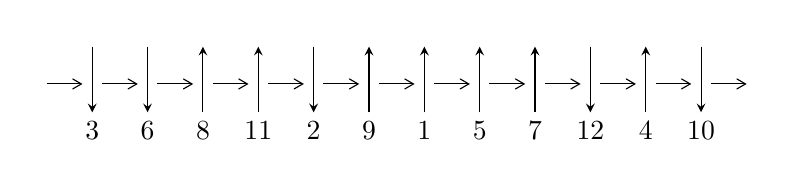
\begin{tikzpicture}[x=20pt, y=17pt]
	% nodes
	\node (C0) at (0, 0) {};
	\node (C1) at (1, 0) {};
	\node (C1U) at (1, +1) {};
	\node (C1D) at (1, -1) {3};

	\node (C2) at (2, 0) {};
	\node (C2U) at (2, +1) {};
	\node (C2D) at (2, -1) {6};

	\node (C3) at (3, 0) {};
	\node (C3U) at (3, +1) {};
	\node (C3D) at (3, -1) {8};

	\node (C4) at (4, 0) {};
	\node (C4U) at (4, +1) {};
	\node (C4D) at (4, -1) {11};

	\node (C5) at (5, 0) {};
	\node (C5U) at (5, +1) {};
	\node (C5D) at (5, -1) {2};

	\node (C6) at (6, 0) {};
	\node (C6U) at (6, +1) {};
	\node (C6D) at (6, -1) {9};

	\node (C7) at (7, 0) {};
	\node (C7U) at (7, +1) {};
	\node (C7D) at (7, -1) {1};

	\node (C8) at (8, 0) {};
	\node (C8U) at (8, +1) {};
	\node (C8D) at (8, -1) {5};

	\node (C9) at (9, 0) {};
	\node (C9U) at (9, +1) {};
	\node (C9D) at (9, -1) {7};

	\node (C10) at (10, 0) {};
	\node (C10U) at (10, +1) {};
	\node (C10D) at (10, -1) {12};

	\node (C11) at (11, 0) {};
	\node (C11U) at (11, +1) {};
	\node (C11D) at (11, -1) {4};

	\node (C12) at (12, 0) {};
	\node (C12U) at (12, +1) {};
	\node (C12D) at (12, -1) {10};
	\node (C13) at (13, 0) {};

	% arrows
	\draw[->,>={angle 60}]
	(C0) edge (C1) (C1) edge (C2) (C2) edge (C3) (C3) edge (C4) (C4) edge (C5) (C5) edge (C6) (C6) edge (C7) (C7) edge (C8) (C8) edge (C9) (C9) edge (C10) (C10) edge (C11) (C11) edge (C12) (C12) edge (C13) ;	\draw[->,>=stealth]
	(C1U) edge (C1D) (C2U) edge (C2D) (C3D) edge (C3U) (C4D) edge (C4U) (C5U) edge (C5D) (C6D) edge (C6U) (C7D) edge (C7U) (C8D) edge (C8U) (C9D) edge (C9U) (C10U) edge (C10D) (C11D) edge (C11U) (C12U) edge (C12D) ;
	\end{tikzpicture} \\
\hhline{~~} \\& 
\textbf{Solving Sequence} \\ \cline{2-2} 
 &
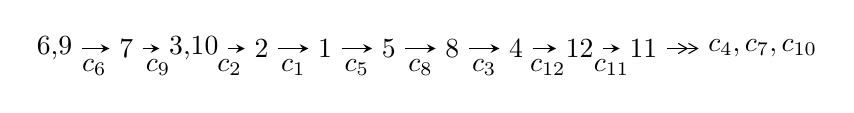
\begin{tikzpicture}[x=23pt, y=7pt]
	% node
	\node (A0) at (-1/8, 0) {6,9};
	\node (A1) at (1, 0) {7};
	\node (A2) at (33/16, 0) {3,10};
	\node (A3) at (25/8, 0) {2};
	\node (A4) at (33/8, 0) {1};
	\node (A5) at (41/8, 0) {5};
	\node (A6) at (49/8, 0) {8};
	\node (A7) at (57/8, 0) {4};
	\node (A8) at (65/8, 0) {12};
	\node (A9) at (73/8, 0) {11};
	\node (C1) at (1/2, -1) {$c_{6}$};
	\node (C2) at (3/2, -1) {$c_{9}$};
	\node (C3) at (21/8, -1) {$c_{2}$};
	\node (C4) at (29/8, -1) {$c_{1}$};
	\node (C5) at (37/8, -1) {$c_{5}$};
	\node (C6) at (45/8, -1) {$c_{8}$};
	\node (C7) at (53/8, -1) {$c_{3}$};
	\node (C8) at (61/8, -1) {$c_{12}$};
	\node (C9) at (69/8, -1) {$c_{11}$};
	\node (A10) at (11, 0) {$c_{4},c_{7},c_{10}$};

	% edge
	\draw[->,>=stealth]	
	(A0) edge (A1) (A1) edge (A2) (A2) edge (A3) (A3) edge (A4) (A4) edge (A5) (A5) edge (A6) (A6) edge (A7) (A7) edge (A8) (A8) edge (A9) ;
	\draw[->>,>={angle 60}]	
	(A9) edge (A10);
\end{tikzpicture} \\ 

\end{tabular} \\

\footnotetext{
The image of knot diagram is generated by the software ``\textbf{Draw programme}" developed by Andrew Bartholomew(\url{http://www.layer8.co.uk/maths/draw/index.htm\#Running-draw}), where we modified some parts for our purpose(\url{https://github.com/CATsTAILs/LinksPainter}).
}\phantom \\ \newline 
\centering \textbf{Ideals for irreducible components\footnotemark of $X_{\text{par}}$} 
 
\begin{align*}
I^u_{1}&=\langle 
-1.25817\times10^{400} u^{103}+6.06573\times10^{400} u^{102}+\cdots+2.71520\times10^{400} b-4.51803\times10^{402},\\
\phantom{I^u_{1}}&\phantom{= \langle  }3.84894\times10^{400} u^{103}-1.79264\times10^{401} u^{102}+\cdots+3.39400\times10^{400} a+2.41261\times10^{403},\\
\phantom{I^u_{1}}&\phantom{= \langle  }u^{104}-6 u^{103}+\cdots-8175 u-625\rangle \\
I^u_{2}&=\langle 
25 a^4-5 a^3+2 a^2+4 b+11 a+3,\;25 a^5-5 a^4+2 a^3+6 a^2+5 a-1,\;u+1\rangle \\
\\
\end{align*}
\raggedright * 2 irreducible components of $\dim_{\mathbb{C}}=0$, with total 109 representations.\\
\footnotetext{All coefficients of polynomials are rational numbers. But the coefficients are sometimes approximated in decimal forms when there is not enough margin.}
\newpage
\renewcommand{\arraystretch}{1}
\centering \section*{I. $I^u_{1}= \langle -1.26\times10^{400} u^{103}+6.07\times10^{400} u^{102}+\cdots+2.72\times10^{400} b-4.52\times10^{402},\;3.85\times10^{400} u^{103}-1.79\times10^{401} u^{102}+\cdots+3.39\times10^{400} a+2.41\times10^{403},\;u^{104}-6 u^{103}+\cdots-8175 u-625 \rangle$}
\flushleft \textbf{(i) Arc colorings}\\
\begin{tabular}{m{7pt} m{180pt} m{7pt} m{180pt} }
\flushright $a_{6}=$&$\begin{pmatrix}1\\0\end{pmatrix}$ \\
\flushright $a_{9}=$&$\begin{pmatrix}0\\u\end{pmatrix}$ \\
\flushright $a_{7}=$&$\begin{pmatrix}1\\- u^2\end{pmatrix}$ \\
\flushright $a_{3}=$&$\begin{pmatrix}-1.13404 u^{103}+5.28179 u^{102}+\cdots-8692.58 u-710.844\\0.463381 u^{103}-2.23399 u^{102}+\cdots+2498.84 u+166.397\end{pmatrix}$ \\
\flushright $a_{10}=$&$\begin{pmatrix}u\\- u^3+u\end{pmatrix}$ \\
\flushright $a_{2}=$&$\begin{pmatrix}-0.670662 u^{103}+3.04780 u^{102}+\cdots-6193.74 u-544.447\\0.463381 u^{103}-2.23399 u^{102}+\cdots+2498.84 u+166.397\end{pmatrix}$ \\
\flushright $a_{1}=$&$\begin{pmatrix}1.07459 u^{103}-5.59952 u^{102}+\cdots-3167.52 u-538.320\\-1.25102 u^{103}+5.81009 u^{102}+\cdots-8824.16 u-651.600\end{pmatrix}$ \\
\flushright $a_{5}=$&$\begin{pmatrix}0.714651 u^{103}-3.81450 u^{102}+\cdots-3127.85 u-359.311\\-1.30915 u^{103}+6.22051 u^{102}+\cdots-7633.41 u-537.319\end{pmatrix}$ \\
\flushright $a_{8}=$&$\begin{pmatrix}-0.384925 u^{103}+2.58489 u^{102}+\cdots+15388.0 u+1690.93\\-0.867986 u^{103}+3.89150 u^{102}+\cdots-6473.36 u-445.958\end{pmatrix}$ \\
\flushright $a_{4}=$&$\begin{pmatrix}-0.591519 u^{103}+2.65264 u^{102}+\cdots-7469.87 u-752.274\\-0.496111 u^{103}+2.31885 u^{102}+\cdots-3046.93 u-227.266\end{pmatrix}$ \\
\flushright $a_{12}=$&$\begin{pmatrix}-0.349150 u^{103}+1.07505 u^{102}+\cdots-11968.9 u-1158.87\\-0.178604 u^{103}+0.831504 u^{102}+\cdots-1466.07 u-104.748\end{pmatrix}$ \\
\flushright $a_{11}=$&$\begin{pmatrix}1.68396 u^{103}-9.20013 u^{102}+\cdots-12447.3 u-1482.86\\-0.498847 u^{103}+2.24348 u^{102}+\cdots-4062.81 u-346.564\end{pmatrix}$\\&\end{tabular}
\flushleft \textbf{(ii) Obstruction class $= -1$}\\~\\
\flushleft \textbf{(iii) Cusp Shapes $= -0.235557 u^{103}+1.17647 u^{102}+\cdots+281.718 u-57.7009$}\\~\\
\newpage\renewcommand{\arraystretch}{1}
\flushleft \textbf{(iv) u-Polynomials at the component}\newline \\
\begin{tabular}{m{50pt}|m{274pt}}
Crossings & \hspace{64pt}u-Polynomials at each crossing \\
\hline $$\begin{aligned}c_{1}\end{aligned}$$&$\begin{aligned}
&u^{104}+42 u^{103}+\cdots+5 u+1
\end{aligned}$\\
\hline $$\begin{aligned}c_{2},c_{5}\end{aligned}$$&$\begin{aligned}
&u^{104}+2 u^{103}+\cdots+u-1
\end{aligned}$\\
\hline $$\begin{aligned}c_{3}\end{aligned}$$&$\begin{aligned}
&u^{104}+u^{103}+\cdots+128000 u+20000
\end{aligned}$\\
\hline $$\begin{aligned}c_{4},c_{11}\end{aligned}$$&$\begin{aligned}
&u^{104}-2 u^{103}+\cdots+3 u-1
\end{aligned}$\\
\hline $$\begin{aligned}c_{6},c_{9}\end{aligned}$$&$\begin{aligned}
&u^{104}+6 u^{103}+\cdots+8175 u-625
\end{aligned}$\\
\hline $$\begin{aligned}c_{7}\end{aligned}$$&$\begin{aligned}
&25(25 u^{104}+125 u^{103}+\cdots-5.04359\times10^{7} u-1.75923\times10^{8})
\end{aligned}$\\
\hline $$\begin{aligned}c_{8}\end{aligned}$$&$\begin{aligned}
&25(25 u^{104}+50 u^{103}+\cdots+4032879 u+1554593)
\end{aligned}$\\
\hline $$\begin{aligned}c_{10},c_{12}\end{aligned}$$&$\begin{aligned}
&u^{104}+30 u^{103}+\cdots-5 u+1
\end{aligned}$\\
\hline
\end{tabular}\\~\\
\newpage\renewcommand{\arraystretch}{1}
\flushleft \textbf{(v) Riley Polynomials at the component}\newline \\
\begin{tabular}{m{50pt}|m{274pt}}
Crossings & \hspace{64pt}Riley Polynomials at each crossing \\
\hline $$\begin{aligned}c_{1}\end{aligned}$$&$\begin{aligned}
&y^{104}+42 y^{103}+\cdots+83 y+1
\end{aligned}$\\
\hline $$\begin{aligned}c_{2},c_{5}\end{aligned}$$&$\begin{aligned}
&y^{104}-42 y^{103}+\cdots-5 y+1
\end{aligned}$\\
\hline $$\begin{aligned}c_{3}\end{aligned}$$&$\begin{aligned}
&y^{104}-33 y^{103}+\cdots-16280000000 y+400000000
\end{aligned}$\\
\hline $$\begin{aligned}c_{4},c_{11}\end{aligned}$$&$\begin{aligned}
&y^{104}+30 y^{103}+\cdots-5 y+1
\end{aligned}$\\
\hline $$\begin{aligned}c_{6},c_{9}\end{aligned}$$&$\begin{aligned}
&y^{104}-86 y^{103}+\cdots-30394375 y+390625
\end{aligned}$\\
\hline $$\begin{aligned}c_{7}\end{aligned}$$&$\begin{aligned}
&625(625 y^{104}-87275 y^{103}+\cdots-7.63958\times10^{17} y+3.09488\times10^{16})
\end{aligned}$\\
\hline $$\begin{aligned}c_{8}\end{aligned}$$&$\begin{aligned}
&625\\
&\cdot(625 y^{104}+16400 y^{103}+\cdots-21479676158875 y+2416759395649)
\end{aligned}$\\
\hline $$\begin{aligned}c_{10},c_{12}\end{aligned}$$&$\begin{aligned}
&y^{104}+90 y^{103}+\cdots-173 y+1
\end{aligned}$\\
\hline
\end{tabular}\\~\\
\newpage\flushleft \textbf{(vi) Complex Volumes and Cusp Shapes}
$$\begin{array}{c|c|c}  
\text{Solutions to }I^u_{1}& \I (\text{vol} + \sqrt{-1}CS) & \text{Cusp shape}\\
 \hline 
\begin{aligned}
u &= -1.013930 + 0.053074 I \\
a &= \phantom{-}0.84563 + 5.97337 I \\
b &= -0.875152 - 0.542840 I\end{aligned}
 & \phantom{-}0.55238 - 2.15431 I & \phantom{-0.000000 } 0 \\ \hline\begin{aligned}
u &= -1.013930 - 0.053074 I \\
a &= \phantom{-}0.84563 - 5.97337 I \\
b &= -0.875152 + 0.542840 I\end{aligned}
 & \phantom{-}0.55238 + 2.15431 I & \phantom{-0.000000 } 0 \\ \hline\begin{aligned}
u &= \phantom{-}1.034930 + 0.092377 I \\
a &= \phantom{-}0.432529 - 0.375380 I \\
b &= -1.43461 + 0.15241 I\end{aligned}
 & -4.20552 + 4.60588 I & \phantom{-0.000000 } 0 \\ \hline\begin{aligned}
u &= \phantom{-}1.034930 - 0.092377 I \\
a &= \phantom{-}0.432529 + 0.375380 I \\
b &= -1.43461 - 0.15241 I\end{aligned}
 & -4.20552 - 4.60588 I & \phantom{-0.000000 } 0 \\ \hline\begin{aligned}
u &= -0.920741 + 0.125206 I \\
a &= -1.26152 - 3.17105 I \\
b &= -0.819156 - 0.413304 I\end{aligned}
 & \phantom{-}4.48936 + 0.62293 I & \phantom{-0.000000 } 0 \\ \hline\begin{aligned}
u &= -0.920741 - 0.125206 I \\
a &= -1.26152 + 3.17105 I \\
b &= -0.819156 + 0.413304 I\end{aligned}
 & \phantom{-}4.48936 - 0.62293 I & \phantom{-0.000000 } 0 \\ \hline\begin{aligned}
u &= \phantom{-}0.025348 + 1.078690 I \\
a &= \phantom{-}0.414738 - 0.689098 I \\
b &= \phantom{-}1.022060 + 0.609154 I\end{aligned}
 & -2.41249 - 7.33475 I & \phantom{-0.000000 } 0 \\ \hline\begin{aligned}
u &= \phantom{-}0.025348 - 1.078690 I \\
a &= \phantom{-}0.414738 + 0.689098 I \\
b &= \phantom{-}1.022060 - 0.609154 I\end{aligned}
 & -2.41249 + 7.33475 I & \phantom{-0.000000 } 0 \\ \hline\begin{aligned}
u &= -1.070450 + 0.147466 I \\
a &= -0.076939 - 0.239125 I \\
b &= -0.140596 - 0.243052 I\end{aligned}
 & \phantom{-}1.177780 - 0.779255 I & \phantom{-0.000000 } 0 \\ \hline\begin{aligned}
u &= -1.070450 - 0.147466 I \\
a &= -0.076939 + 0.239125 I \\
b &= -0.140596 + 0.243052 I\end{aligned}
 & \phantom{-}1.177780 + 0.779255 I & \phantom{-0.000000 } 0\\
 \hline 
 \end{array}$$\newpage$$\begin{array}{c|c|c}  
\text{Solutions to }I^u_{1}& \I (\text{vol} + \sqrt{-1}CS) & \text{Cusp shape}\\
 \hline 
\begin{aligned}
u &= \phantom{-}0.110220 + 0.892342 I \\
a &= -0.914702 - 1.076450 I \\
b &= -1.003870 + 0.038005 I\end{aligned}
 & \phantom{-}0.18628 - 5.77200 I & \phantom{-0.000000 } 0 \\ \hline\begin{aligned}
u &= \phantom{-}0.110220 - 0.892342 I \\
a &= -0.914702 + 1.076450 I \\
b &= -1.003870 - 0.038005 I\end{aligned}
 & \phantom{-}0.18628 + 5.77200 I & \phantom{-0.000000 } 0 \\ \hline\begin{aligned}
u &= -0.867570 + 0.211578 I \\
a &= \phantom{-}1.23556 + 2.33717 I \\
b &= \phantom{-}0.801312 + 0.374759 I\end{aligned}
 & \phantom{-}4.32881 - 5.13184 I & \phantom{-0.000000 } 0 \\ \hline\begin{aligned}
u &= -0.867570 - 0.211578 I \\
a &= \phantom{-}1.23556 - 2.33717 I \\
b &= \phantom{-}0.801312 - 0.374759 I\end{aligned}
 & \phantom{-}4.32881 + 5.13184 I & \phantom{-0.000000 } 0 \\ \hline\begin{aligned}
u &= -0.716194 + 0.516260 I \\
a &= \phantom{-}0.058650 - 0.780537 I \\
b &= -0.439288 - 0.400367 I\end{aligned}
 & \phantom{-}4.70460 + 0.58481 I & \phantom{-0.000000 } 0 \\ \hline\begin{aligned}
u &= -0.716194 - 0.516260 I \\
a &= \phantom{-}0.058650 + 0.780537 I \\
b &= -0.439288 + 0.400367 I\end{aligned}
 & \phantom{-}4.70460 - 0.58481 I & \phantom{-0.000000 } 0 \\ \hline\begin{aligned}
u &= -0.134970 + 0.860713 I \\
a &= \phantom{-}0.305814 + 0.661002 I \\
b &= \phantom{-}0.532236 - 0.624590 I\end{aligned}
 & -1.02515 - 2.43506 I & \phantom{-0.000000 } 0 \\ \hline\begin{aligned}
u &= -0.134970 - 0.860713 I \\
a &= \phantom{-}0.305814 - 0.661002 I \\
b &= \phantom{-}0.532236 + 0.624590 I\end{aligned}
 & -1.02515 + 2.43506 I & \phantom{-0.000000 } 0 \\ \hline\begin{aligned}
u &= \phantom{-}0.755968 + 0.378816 I \\
a &= \phantom{-}0.009408 - 0.920023 I \\
b &= -1.187370 + 0.198303 I\end{aligned}
 & -4.14345 + 4.96463 I & \phantom{-0.000000 } 0 \\ \hline\begin{aligned}
u &= \phantom{-}0.755968 - 0.378816 I \\
a &= \phantom{-}0.009408 + 0.920023 I \\
b &= -1.187370 - 0.198303 I\end{aligned}
 & -4.14345 - 4.96463 I & \phantom{-0.000000 } 0\\
 \hline 
 \end{array}$$\newpage$$\begin{array}{c|c|c}  
\text{Solutions to }I^u_{1}& \I (\text{vol} + \sqrt{-1}CS) & \text{Cusp shape}\\
 \hline 
\begin{aligned}
u &= \phantom{-}1.15916\phantom{ +0.000000I} \\
a &= -0.248154\phantom{ +0.000000I} \\
b &= \phantom{-}1.39516\phantom{ +0.000000I}\end{aligned}
 & -0.196484\phantom{ +0.000000I} & \phantom{-0.000000 } 0 \\ \hline\begin{aligned}
u &= -0.234959 + 0.795544 I \\
a &= -0.790804 + 0.597039 I \\
b &= -0.992648 - 0.590040 I\end{aligned}
 & \phantom{-}0.32570 - 4.74919 I & \phantom{-0.000000 } 0 \\ \hline\begin{aligned}
u &= -0.234959 - 0.795544 I \\
a &= -0.790804 - 0.597039 I \\
b &= -0.992648 + 0.590040 I\end{aligned}
 & \phantom{-}0.32570 + 4.74919 I & \phantom{-0.000000 } 0 \\ \hline\begin{aligned}
u &= \phantom{-}0.031293 + 0.813655 I \\
a &= \phantom{-}0.98332 + 1.14454 I \\
b &= \phantom{-}0.973040 - 0.042367 I\end{aligned}
 & \phantom{-}0.753256 + 0.017776 I & \phantom{-0.000000 } 0 \\ \hline\begin{aligned}
u &= \phantom{-}0.031293 - 0.813655 I \\
a &= \phantom{-}0.98332 - 1.14454 I \\
b &= \phantom{-}0.973040 + 0.042367 I\end{aligned}
 & \phantom{-}0.753256 - 0.017776 I & \phantom{-0.000000 } 0 \\ \hline\begin{aligned}
u &= \phantom{-}0.400031 + 0.699404 I \\
a &= -0.568973 - 1.153310 I \\
b &= -1.058270 + 0.115697 I\end{aligned}
 & -5.49838 - 1.03204 I & \phantom{-0.000000 } 0 \\ \hline\begin{aligned}
u &= \phantom{-}0.400031 - 0.699404 I \\
a &= -0.568973 + 1.153310 I \\
b &= -1.058270 - 0.115697 I\end{aligned}
 & -5.49838 + 1.03204 I & \phantom{-0.000000 } 0 \\ \hline\begin{aligned}
u &= -0.608735 + 0.525411 I \\
a &= -0.166435 + 0.966502 I \\
b &= \phantom{-}0.490251 + 0.429515 I\end{aligned}
 & \phantom{-}4.41771 - 5.22605 I & \phantom{-0.000000 } 0 \\ \hline\begin{aligned}
u &= -0.608735 - 0.525411 I \\
a &= -0.166435 - 0.966502 I \\
b &= \phantom{-}0.490251 - 0.429515 I\end{aligned}
 & \phantom{-}4.41771 + 5.22605 I & \phantom{-0.000000 } 0 \\ \hline\begin{aligned}
u &= -0.517612 + 0.557275 I \\
a &= -0.267475 - 0.044433 I \\
b &= -0.631086 + 0.547783 I\end{aligned}
 & \phantom{-}1.42679 - 0.09115 I & \phantom{-}8.32769 + 0. I\phantom{ +0.000000I}\\
 \hline 
 \end{array}$$\newpage$$\begin{array}{c|c|c}  
\text{Solutions to }I^u_{1}& \I (\text{vol} + \sqrt{-1}CS) & \text{Cusp shape}\\
 \hline 
\begin{aligned}
u &= -0.517612 - 0.557275 I \\
a &= -0.267475 + 0.044433 I \\
b &= -0.631086 - 0.547783 I\end{aligned}
 & \phantom{-}1.42679 + 0.09115 I & \phantom{-}8.32769 + 0. I\phantom{ +0.000000I} \\ \hline\begin{aligned}
u &= \phantom{-}1.249050 + 0.091321 I \\
a &= -0.63785 - 1.27059 I \\
b &= \phantom{-}0.541821 + 1.005770 I\end{aligned}
 & \phantom{-}3.02371 - 1.07462 I & \phantom{-0.000000 } 0 \\ \hline\begin{aligned}
u &= \phantom{-}1.249050 - 0.091321 I \\
a &= -0.63785 + 1.27059 I \\
b &= \phantom{-}0.541821 - 1.005770 I\end{aligned}
 & \phantom{-}3.02371 + 1.07462 I & \phantom{-0.000000 } 0 \\ \hline\begin{aligned}
u &= \phantom{-}1.230010 + 0.257322 I \\
a &= -0.18469 + 1.76690 I \\
b &= \phantom{-}1.122190 - 0.745710 I\end{aligned}
 & \phantom{-}1.24341 + 5.25068 I & \phantom{-0.000000 } 0 \\ \hline\begin{aligned}
u &= \phantom{-}1.230010 - 0.257322 I \\
a &= -0.18469 - 1.76690 I \\
b &= \phantom{-}1.122190 + 0.745710 I\end{aligned}
 & \phantom{-}1.24341 - 5.25068 I & \phantom{-0.000000 } 0 \\ \hline\begin{aligned}
u &= -0.714203\phantom{ +0.000000I} \\
a &= -0.630403\phantom{ +0.000000I} \\
b &= -0.398199\phantom{ +0.000000I}\end{aligned}
 & \phantom{-}1.03446\phantom{ +0.000000I} & \phantom{-}10.5160\phantom{ +0.000000I} \\ \hline\begin{aligned}
u &= -0.501535 + 1.223320 I \\
a &= -0.021136 - 0.607600 I \\
b &= -0.613344 + 0.675383 I\end{aligned}
 & \phantom{-}5.49142 - 0.54714 I & \phantom{-0.000000 } 0 \\ \hline\begin{aligned}
u &= -0.501535 - 1.223320 I \\
a &= -0.021136 + 0.607600 I \\
b &= -0.613344 - 0.675383 I\end{aligned}
 & \phantom{-}5.49142 + 0.54714 I & \phantom{-0.000000 } 0 \\ \hline\begin{aligned}
u &= -0.391187 + 1.267150 I \\
a &= \phantom{-}0.044961 + 0.643911 I \\
b &= \phantom{-}0.598753 - 0.683955 I\end{aligned}
 & \phantom{-}5.05098 - 6.49860 I & \phantom{-0.000000 } 0 \\ \hline\begin{aligned}
u &= -0.391187 - 1.267150 I \\
a &= \phantom{-}0.044961 - 0.643911 I \\
b &= \phantom{-}0.598753 + 0.683955 I\end{aligned}
 & \phantom{-}5.05098 + 6.49860 I & \phantom{-0.000000 } 0\\
 \hline 
 \end{array}$$\newpage$$\begin{array}{c|c|c}  
\text{Solutions to }I^u_{1}& \I (\text{vol} + \sqrt{-1}CS) & \text{Cusp shape}\\
 \hline 
\begin{aligned}
u &= \phantom{-}1.327230 + 0.025075 I \\
a &= -0.20990 - 1.43950 I \\
b &= \phantom{-}1.169970 + 0.711145 I\end{aligned}
 & \phantom{-}8.34639 + 1.35481 I & \phantom{-0.000000 } 0 \\ \hline\begin{aligned}
u &= \phantom{-}1.327230 - 0.025075 I \\
a &= -0.20990 + 1.43950 I \\
b &= \phantom{-}1.169970 - 0.711145 I\end{aligned}
 & \phantom{-}8.34639 - 1.35481 I & \phantom{-0.000000 } 0 \\ \hline\begin{aligned}
u &= \phantom{-}1.299360 + 0.322093 I \\
a &= \phantom{-}0.106462 + 0.307157 I \\
b &= \phantom{-}1.284080 - 0.060470 I\end{aligned}
 & \phantom{-}4.83167 + 3.98855 I & \phantom{-0.000000 } 0 \\ \hline\begin{aligned}
u &= \phantom{-}1.299360 - 0.322093 I \\
a &= \phantom{-}0.106462 - 0.307157 I \\
b &= \phantom{-}1.284080 + 0.060470 I\end{aligned}
 & \phantom{-}4.83167 - 3.98855 I & \phantom{-0.000000 } 0 \\ \hline\begin{aligned}
u &= -1.157470 + 0.677359 I \\
a &= -0.43424 + 1.62457 I \\
b &= -0.918558 - 0.625354 I\end{aligned}
 & \phantom{-}2.25024 - 5.42318 I & \phantom{-0.000000 } 0 \\ \hline\begin{aligned}
u &= -1.157470 - 0.677359 I \\
a &= -0.43424 - 1.62457 I \\
b &= -0.918558 + 0.625354 I\end{aligned}
 & \phantom{-}2.25024 + 5.42318 I & \phantom{-0.000000 } 0 \\ \hline\begin{aligned}
u &= -1.247090 + 0.519183 I \\
a &= \phantom{-}0.653265 - 0.592996 I \\
b &= -0.753696 + 0.620768 I\end{aligned}
 & \phantom{-}2.75612 - 0.51612 I & \phantom{-0.000000 } 0 \\ \hline\begin{aligned}
u &= -1.247090 - 0.519183 I \\
a &= \phantom{-}0.653265 + 0.592996 I \\
b &= -0.753696 - 0.620768 I\end{aligned}
 & \phantom{-}2.75612 + 0.51612 I & \phantom{-0.000000 } 0 \\ \hline\begin{aligned}
u &= \phantom{-}1.293830 + 0.393590 I \\
a &= -0.149281 - 0.351146 I \\
b &= -1.270650 + 0.063796 I\end{aligned}
 & \phantom{-}4.02286 + 10.36490 I & \phantom{-0.000000 } 0 \\ \hline\begin{aligned}
u &= \phantom{-}1.293830 - 0.393590 I \\
a &= -0.149281 + 0.351146 I \\
b &= -1.270650 - 0.063796 I\end{aligned}
 & \phantom{-}4.02286 - 10.36490 I & \phantom{-0.000000 } 0\\
 \hline 
 \end{array}$$\newpage$$\begin{array}{c|c|c}  
\text{Solutions to }I^u_{1}& \I (\text{vol} + \sqrt{-1}CS) & \text{Cusp shape}\\
 \hline 
\begin{aligned}
u &= -1.366010 + 0.033928 I \\
a &= \phantom{-}0.001319 - 0.235797 I \\
b &= -0.015035 - 0.391381 I\end{aligned}
 & \phantom{-}6.33487 - 2.95650 I & \phantom{-0.000000 } 0 \\ \hline\begin{aligned}
u &= -1.366010 - 0.033928 I \\
a &= \phantom{-}0.001319 + 0.235797 I \\
b &= -0.015035 + 0.391381 I\end{aligned}
 & \phantom{-}6.33487 + 2.95650 I & \phantom{-0.000000 } 0 \\ \hline\begin{aligned}
u &= -0.532280 + 0.337940 I \\
a &= \phantom{-}1.072810 + 0.907460 I \\
b &= \phantom{-}0.641319 + 0.116720 I\end{aligned}
 & -0.95235 - 1.78350 I & -2.07327 + 5.75596 I \\ \hline\begin{aligned}
u &= -0.532280 - 0.337940 I \\
a &= \phantom{-}1.072810 - 0.907460 I \\
b &= \phantom{-}0.641319 - 0.116720 I\end{aligned}
 & -0.95235 + 1.78350 I & -2.07327 - 5.75596 I \\ \hline\begin{aligned}
u &= \phantom{-}1.325390 + 0.351138 I \\
a &= -0.775024 - 1.068110 I \\
b &= \phantom{-}0.561537 + 0.938182 I\end{aligned}
 & \phantom{-}3.49061 + 6.69572 I & \phantom{-0.000000 } 0 \\ \hline\begin{aligned}
u &= \phantom{-}1.325390 - 0.351138 I \\
a &= -0.775024 + 1.068110 I \\
b &= \phantom{-}0.561537 - 0.938182 I\end{aligned}
 & \phantom{-}3.49061 - 6.69572 I & \phantom{-0.000000 } 0 \\ \hline\begin{aligned}
u &= \phantom{-}1.373980 + 0.047061 I \\
a &= \phantom{-}0.15734 - 1.49974 I \\
b &= -1.155940 + 0.715392 I\end{aligned}
 & \phantom{-}9.36202 + 5.02654 I & \phantom{-0.000000 } 0 \\ \hline\begin{aligned}
u &= \phantom{-}1.373980 - 0.047061 I \\
a &= \phantom{-}0.15734 + 1.49974 I \\
b &= -1.155940 - 0.715392 I\end{aligned}
 & \phantom{-}9.36202 - 5.02654 I & \phantom{-0.000000 } 0 \\ \hline\begin{aligned}
u &= \phantom{-}1.380450 + 0.205876 I \\
a &= \phantom{-}0.668151 + 1.119090 I \\
b &= -0.541182 - 0.958954 I\end{aligned}
 & \phantom{-}7.11860 + 2.72109 I & \phantom{-0.000000 } 0 \\ \hline\begin{aligned}
u &= \phantom{-}1.380450 - 0.205876 I \\
a &= \phantom{-}0.668151 - 1.119090 I \\
b &= -0.541182 + 0.958954 I\end{aligned}
 & \phantom{-}7.11860 - 2.72109 I & \phantom{-0.000000 } 0\\
 \hline 
 \end{array}$$\newpage$$\begin{array}{c|c|c}  
\text{Solutions to }I^u_{1}& \I (\text{vol} + \sqrt{-1}CS) & \text{Cusp shape}\\
 \hline 
\begin{aligned}
u &= \phantom{-}1.399670 + 0.162927 I \\
a &= -0.419135 + 1.168260 I \\
b &= \phantom{-}0.473091 - 0.966081 I\end{aligned}
 & \phantom{-}10.46890 + 7.48108 I & \phantom{-0.000000 } 0 \\ \hline\begin{aligned}
u &= \phantom{-}1.399670 - 0.162927 I \\
a &= -0.419135 - 1.168260 I \\
b &= \phantom{-}0.473091 + 0.966081 I\end{aligned}
 & \phantom{-}10.46890 - 7.48108 I & \phantom{-0.000000 } 0 \\ \hline\begin{aligned}
u &= -1.386420 + 0.266585 I \\
a &= -0.25593 - 1.81404 I \\
b &= \phantom{-}0.869849 + 0.621736 I\end{aligned}
 & \phantom{-}3.35689 - 2.65952 I & \phantom{-0.000000 } 0 \\ \hline\begin{aligned}
u &= -1.386420 - 0.266585 I \\
a &= -0.25593 + 1.81404 I \\
b &= \phantom{-}0.869849 - 0.621736 I\end{aligned}
 & \phantom{-}3.35689 + 2.65952 I & \phantom{-0.000000 } 0 \\ \hline\begin{aligned}
u &= \phantom{-}1.37389 + 0.33988 I \\
a &= \phantom{-}0.02125 - 1.72170 I \\
b &= -1.118940 + 0.720663 I\end{aligned}
 & \phantom{-}5.34196 + 8.84585 I & \phantom{-0.000000 } 0 \\ \hline\begin{aligned}
u &= \phantom{-}1.37389 - 0.33988 I \\
a &= \phantom{-}0.02125 + 1.72170 I \\
b &= -1.118940 - 0.720663 I\end{aligned}
 & \phantom{-}5.34196 - 8.84585 I & \phantom{-0.000000 } 0 \\ \hline\begin{aligned}
u &= -0.28820 + 1.38713 I \\
a &= -0.446882 + 0.904495 I \\
b &= -1.003300 - 0.636591 I\end{aligned}
 & \phantom{-}4.34614 - 5.65703 I & \phantom{-0.000000 } 0 \\ \hline\begin{aligned}
u &= -0.28820 - 1.38713 I \\
a &= -0.446882 - 0.904495 I \\
b &= -1.003300 + 0.636591 I\end{aligned}
 & \phantom{-}4.34614 + 5.65703 I & \phantom{-0.000000 } 0 \\ \hline\begin{aligned}
u &= \phantom{-}1.34330 + 0.47281 I \\
a &= \phantom{-}0.05769 + 1.81023 I \\
b &= \phantom{-}1.105550 - 0.715397 I\end{aligned}
 & \phantom{-}1.81081 + 12.75050 I & \phantom{-0.000000 } 0 \\ \hline\begin{aligned}
u &= \phantom{-}1.34330 - 0.47281 I \\
a &= \phantom{-}0.05769 - 1.81023 I \\
b &= \phantom{-}1.105550 + 0.715397 I\end{aligned}
 & \phantom{-}1.81081 - 12.75050 I & \phantom{-0.000000 } 0\\
 \hline 
 \end{array}$$\newpage$$\begin{array}{c|c|c}  
\text{Solutions to }I^u_{1}& \I (\text{vol} + \sqrt{-1}CS) & \text{Cusp shape}\\
 \hline 
\begin{aligned}
u &= \phantom{-}1.43078 + 0.09268 I \\
a &= \phantom{-}0.463511 - 1.152510 I \\
b &= -0.487227 + 0.966447 I\end{aligned}
 & \phantom{-}11.40100 + 1.10913 I & \phantom{-0.000000 } 0 \\ \hline\begin{aligned}
u &= \phantom{-}1.43078 - 0.09268 I \\
a &= \phantom{-}0.463511 + 1.152510 I \\
b &= -0.487227 - 0.966447 I\end{aligned}
 & \phantom{-}11.40100 - 1.10913 I & \phantom{-0.000000 } 0 \\ \hline\begin{aligned}
u &= -0.18781 + 1.43114 I \\
a &= \phantom{-}0.413662 - 0.884510 I \\
b &= \phantom{-}1.010510 + 0.637829 I\end{aligned}
 & \phantom{-}3.84645 - 11.63360 I & \phantom{-0.000000 } 0 \\ \hline\begin{aligned}
u &= -0.18781 - 1.43114 I \\
a &= \phantom{-}0.413662 + 0.884510 I \\
b &= \phantom{-}1.010510 - 0.637829 I\end{aligned}
 & \phantom{-}3.84645 + 11.63360 I & \phantom{-0.000000 } 0 \\ \hline\begin{aligned}
u &= -1.44555 + 0.08629 I \\
a &= -0.74940 + 1.33777 I \\
b &= \phantom{-}0.823412 - 0.622826 I\end{aligned}
 & \phantom{-}3.50118 + 2.22683 I & \phantom{-0.000000 } 0 \\ \hline\begin{aligned}
u &= -1.44555 - 0.08629 I \\
a &= -0.74940 - 1.33777 I \\
b &= \phantom{-}0.823412 + 0.622826 I\end{aligned}
 & \phantom{-}3.50118 - 2.22683 I & \phantom{-0.000000 } 0 \\ \hline\begin{aligned}
u &= \phantom{-}0.190949 + 0.516496 I \\
a &= \phantom{-}0.0145879 - 0.0144478 I \\
b &= \phantom{-}1.031680 + 0.541785 I\end{aligned}
 & -2.05610 - 2.20533 I & -3.33452 - 0.09970 I \\ \hline\begin{aligned}
u &= \phantom{-}0.190949 - 0.516496 I \\
a &= \phantom{-}0.0145879 + 0.0144478 I \\
b &= \phantom{-}1.031680 - 0.541785 I\end{aligned}
 & -2.05610 + 2.20533 I & -3.33452 + 0.09970 I \\ \hline\begin{aligned}
u &= \phantom{-}0.345318 + 0.335466 I \\
a &= \phantom{-}0.12836 + 1.71447 I \\
b &= \phantom{-}1.029410 - 0.244500 I\end{aligned}
 & -1.96391 + 1.11544 I & -1.55787 - 1.47213 I \\ \hline\begin{aligned}
u &= \phantom{-}0.345318 - 0.335466 I \\
a &= \phantom{-}0.12836 - 1.71447 I \\
b &= \phantom{-}1.029410 + 0.244500 I\end{aligned}
 & -1.96391 - 1.11544 I & -1.55787 + 1.47213 I\\
 \hline 
 \end{array}$$\newpage$$\begin{array}{c|c|c}  
\text{Solutions to }I^u_{1}& \I (\text{vol} + \sqrt{-1}CS) & \text{Cusp shape}\\
 \hline 
\begin{aligned}
u &= \phantom{-}0.370544 + 0.231620 I \\
a &= \phantom{-}0.30459 + 1.57062 I \\
b &= \phantom{-}0.178701 - 0.619565 I\end{aligned}
 & \phantom{-}0.02077 + 2.00050 I & -0.12885 - 4.33329 I \\ \hline\begin{aligned}
u &= \phantom{-}0.370544 - 0.231620 I \\
a &= \phantom{-}0.30459 - 1.57062 I \\
b &= \phantom{-}0.178701 + 0.619565 I\end{aligned}
 & \phantom{-}0.02077 - 2.00050 I & -0.12885 + 4.33329 I \\ \hline\begin{aligned}
u &= \phantom{-}1.51573 + 0.42036 I \\
a &= \phantom{-}0.698231 + 0.961625 I \\
b &= -0.536978 - 0.923935 I\end{aligned}
 & \phantom{-}11.80750 + 6.14222 I & \phantom{-0.000000 } 0 \\ \hline\begin{aligned}
u &= \phantom{-}1.51573 - 0.42036 I \\
a &= \phantom{-}0.698231 - 0.961625 I \\
b &= -0.536978 + 0.923935 I\end{aligned}
 & \phantom{-}11.80750 - 6.14222 I & \phantom{-0.000000 } 0 \\ \hline\begin{aligned}
u &= \phantom{-}1.50371 + 0.47064 I \\
a &= -0.717795 - 0.941657 I \\
b &= \phantom{-}0.538804 + 0.918861 I\end{aligned}
 & \phantom{-}10.9616 + 12.4442 I & \phantom{-0.000000 } 0 \\ \hline\begin{aligned}
u &= \phantom{-}1.50371 - 0.47064 I \\
a &= -0.717795 + 0.941657 I \\
b &= \phantom{-}0.538804 - 0.918861 I\end{aligned}
 & \phantom{-}10.9616 - 12.4442 I & \phantom{-0.000000 } 0 \\ \hline\begin{aligned}
u &= -0.422179 + 0.033106 I \\
a &= -4.10481 - 1.84710 I \\
b &= -0.946056 + 0.550739 I\end{aligned}
 & \phantom{-}3.70136 + 4.72366 I & \phantom{-}5.70262 - 6.08247 I \\ \hline\begin{aligned}
u &= -0.422179 - 0.033106 I \\
a &= -4.10481 + 1.84710 I \\
b &= -0.946056 - 0.550739 I\end{aligned}
 & \phantom{-}3.70136 - 4.72366 I & \phantom{-}5.70262 + 6.08247 I \\ \hline\begin{aligned}
u &= \phantom{-}1.51283 + 0.51617 I \\
a &= -0.14872 - 1.71406 I \\
b &= -1.112300 + 0.702932 I\end{aligned}
 & \phantom{-}10.0427 + 12.1163 I & \phantom{-0.000000 } 0 \\ \hline\begin{aligned}
u &= \phantom{-}1.51283 - 0.51617 I \\
a &= -0.14872 + 1.71406 I \\
b &= -1.112300 - 0.702932 I\end{aligned}
 & \phantom{-}10.0427 - 12.1163 I & \phantom{-0.000000 } 0\\
 \hline 
 \end{array}$$\newpage$$\begin{array}{c|c|c}  
\text{Solutions to }I^u_{1}& \I (\text{vol} + \sqrt{-1}CS) & \text{Cusp shape}\\
 \hline 
\begin{aligned}
u &= \phantom{-}1.50426 + 0.56043 I \\
a &= \phantom{-}0.17208 + 1.73252 I \\
b &= \phantom{-}1.109870 - 0.701364 I\end{aligned}
 & \phantom{-}9.2104 + 18.3996 I & \phantom{-0.000000 } 0 \\ \hline\begin{aligned}
u &= \phantom{-}1.50426 - 0.56043 I \\
a &= \phantom{-}0.17208 - 1.73252 I \\
b &= \phantom{-}1.109870 + 0.701364 I\end{aligned}
 & \phantom{-}9.2104 - 18.3996 I & \phantom{-0.000000 } 0 \\ \hline\begin{aligned}
u &= -0.275966 + 0.081922 I \\
a &= \phantom{-}5.36153 + 2.17952 I \\
b &= \phantom{-}0.942019 - 0.553208 I\end{aligned}
 & \phantom{-}3.44019 - 0.96910 I & \phantom{-}4.29951 - 0.42121 I \\ \hline\begin{aligned}
u &= -0.275966 - 0.081922 I \\
a &= \phantom{-}5.36153 - 2.17952 I \\
b &= \phantom{-}0.942019 + 0.553208 I\end{aligned}
 & \phantom{-}3.44019 + 0.96910 I & \phantom{-}4.29951 + 0.42121 I \\ \hline\begin{aligned}
u &= -0.258260 + 0.055783 I \\
a &= \phantom{-}2.30549 - 2.00942 I \\
b &= \phantom{-}0.703307 - 0.430355 I\end{aligned}
 & -0.81820 + 1.73592 I & -0.97741 - 5.34079 I \\ \hline\begin{aligned}
u &= -0.258260 - 0.055783 I \\
a &= \phantom{-}2.30549 + 2.00942 I \\
b &= \phantom{-}0.703307 + 0.430355 I\end{aligned}
 & -0.81820 - 1.73592 I & -0.97741 + 5.34079 I \\ \hline\begin{aligned}
u &= -1.67498 + 0.83826 I \\
a &= -0.128673 + 1.344690 I \\
b &= -0.905498 - 0.666581 I\end{aligned}
 & \phantom{-}8.57816 - 8.03076 I & \phantom{-0.000000 } 0 \\ \hline\begin{aligned}
u &= -1.67498 - 0.83826 I \\
a &= -0.128673 - 1.344690 I \\
b &= -0.905498 + 0.666581 I\end{aligned}
 & \phantom{-}8.57816 + 8.03076 I & \phantom{-0.000000 } 0 \\ \hline\begin{aligned}
u &= -1.78021 + 0.60840 I \\
a &= \phantom{-}0.370721 - 0.903073 I \\
b &= -0.781342 + 0.678105 I\end{aligned}
 & \phantom{-}8.95454 - 2.83317 I & \phantom{-0.000000 } 0 \\ \hline\begin{aligned}
u &= -1.78021 - 0.60840 I \\
a &= \phantom{-}0.370721 + 0.903073 I \\
b &= -0.781342 - 0.678105 I\end{aligned}
 & \phantom{-}8.95454 + 2.83317 I & \phantom{-0.000000 } 0\\
 \hline 
 \end{array}$$\newpage$$\begin{array}{c|c|c}  
\text{Solutions to }I^u_{1}& \I (\text{vol} + \sqrt{-1}CS) & \text{Cusp shape}\\
 \hline 
\begin{aligned}
u &= -1.72719 + 0.74945 I \\
a &= \phantom{-}0.080288 - 1.352320 I \\
b &= \phantom{-}0.898221 + 0.667170 I\end{aligned}
 & \phantom{-}8.74433 - 1.97763 I & \phantom{-0.000000 } 0 \\ \hline\begin{aligned}
u &= -1.72719 - 0.74945 I \\
a &= \phantom{-}0.080288 + 1.352320 I \\
b &= \phantom{-}0.898221 - 0.667170 I\end{aligned}
 & \phantom{-}8.74433 + 1.97763 I & \phantom{-0.000000 } 0 \\ \hline\begin{aligned}
u &= -1.82306 + 0.51731 I \\
a &= -0.372352 + 0.949139 I \\
b &= \phantom{-}0.790607 - 0.677284 I\end{aligned}
 & \phantom{-}9.07102 + 3.21849 I & \phantom{-0.000000 } 0 \\ \hline\begin{aligned}
u &= -1.82306 - 0.51731 I \\
a &= -0.372352 - 0.949139 I \\
b &= \phantom{-}0.790607 + 0.677284 I\end{aligned}
 & \phantom{-}9.07102 - 3.21849 I & \phantom{-0.000000 } 0\\
 \hline 
 \end{array}$$\newpage\newpage\renewcommand{\arraystretch}{1}
\centering \section*{II. $I^u_{2}= \langle 25 a^4-5 a^3+2 a^2+4 b+11 a+3,\;25 a^5-5 a^4+2 a^3+6 a^2+5 a-1,\;u+1 \rangle$}
\flushleft \textbf{(i) Arc colorings}\\
\begin{tabular}{m{7pt} m{180pt} m{7pt} m{180pt} }
\flushright $a_{6}=$&$\begin{pmatrix}1\\0\end{pmatrix}$ \\
\flushright $a_{9}=$&$\begin{pmatrix}0\\-1\end{pmatrix}$ \\
\flushright $a_{7}=$&$\begin{pmatrix}1\\-1\end{pmatrix}$ \\
\flushright $a_{3}=$&$\begin{pmatrix}a\\-\frac{25}{4} a^4+\frac{5}{4} a^3+\cdots-\frac{11}{4} a-\frac{3}{4}\end{pmatrix}$ \\
\flushright $a_{10}=$&$\begin{pmatrix}-1\\0\end{pmatrix}$ \\
\flushright $a_{2}=$&$\begin{pmatrix}-\frac{25}{4} a^4+\frac{5}{4} a^3+\cdots-\frac{7}{4} a-\frac{3}{4}\\-\frac{25}{4} a^4+\frac{5}{4} a^3+\cdots-\frac{11}{4} a-\frac{3}{4}\end{pmatrix}$ \\
\flushright $a_{1}=$&$\begin{pmatrix}-\frac{125}{16} a^4+\frac{5}{8} a^2-3 a-\frac{13}{16}\\\frac{75}{16} a^4+\frac{5}{8} a^3+\cdots+\frac{15}{8} a+\frac{5}{16}\end{pmatrix}$ \\
\flushright $a_{5}=$&$\begin{pmatrix}-\frac{25}{16} a^4-\frac{5}{4} a^3+\cdots+\frac{1}{4} a-\frac{5}{16}\\-\frac{25}{16} a^4-\frac{5}{4} a^3+\cdots+\frac{3}{4} a-\frac{25}{16}\end{pmatrix}$ \\
\flushright $a_{8}=$&$\begin{pmatrix}-\frac{25}{16} a^4-\frac{5}{8} a^3+\frac{1}{8} a+\frac{1}{16}\\-\frac{1}{2} a-\frac{1}{2}\end{pmatrix}$ \\
\flushright $a_{4}=$&$\begin{pmatrix}a\\-\frac{25}{4} a^4+\frac{5}{4} a^3+\cdots-\frac{11}{4} a-\frac{3}{4}\end{pmatrix}$ \\
\flushright $a_{12}=$&$\begin{pmatrix}-\frac{25}{8} a^4+\frac{5}{8} a^3+\cdots-\frac{9}{8} a-\frac{1}{2}\\\frac{75}{16} a^4+\frac{5}{8} a^3+\cdots+\frac{15}{8} a+\frac{5}{16}\end{pmatrix}$ \\
\flushright $a_{11}=$&$\begin{pmatrix}-\frac{1}{2} a-\frac{1}{2}\\-\frac{25}{8} a^4+\frac{15}{4} a^3+\cdots+\frac{3}{4} a-\frac{3}{8}\end{pmatrix}$\\&\end{tabular}
\flushleft \textbf{(ii) Obstruction class $= 1$}\\~\\
\flushleft \textbf{(iii) Cusp Shapes $= -\frac{525}{16} a^4+\frac{105}{4} a^3-\frac{139}{8} a^2+\frac{27}{4} a-\frac{13}{16}$}\\~\\
\newpage\renewcommand{\arraystretch}{1}
\flushleft \textbf{(iv) u-Polynomials at the component}\newline \\
\begin{tabular}{m{50pt}|m{274pt}}
Crossings & \hspace{64pt}u-Polynomials at each crossing \\
\hline $$\begin{aligned}c_{1}\end{aligned}$$&$\begin{aligned}
&u^5-5 u^4+8 u^3-3 u^2- u-1
\end{aligned}$\\
\hline $$\begin{aligned}c_{2}\end{aligned}$$&$\begin{aligned}
&u^5+u^4-2 u^3- u^2+u-1
\end{aligned}$\\
\hline $$\begin{aligned}c_{3}\end{aligned}$$&$\begin{aligned}
&u^5
\end{aligned}$\\
\hline $$\begin{aligned}c_{4}\end{aligned}$$&$\begin{aligned}
&u^5+u^4+2 u^3+u^2+u+1
\end{aligned}$\\
\hline $$\begin{aligned}c_{5}\end{aligned}$$&$\begin{aligned}
&u^5- u^4-2 u^3+u^2+u+1
\end{aligned}$\\
\hline $$\begin{aligned}c_{6}\end{aligned}$$&$\begin{aligned}
&(u+1)^5
\end{aligned}$\\
\hline $$\begin{aligned}c_{7}\end{aligned}$$&$\begin{aligned}
&25(25 u^5-3 u^3+2 u^2-2 u+1)
\end{aligned}$\\
\hline $$\begin{aligned}c_{8}\end{aligned}$$&$\begin{aligned}
&25(25 u^5-25 u^4-17 u^3+10 u^2+7 u+1)
\end{aligned}$\\
\hline $$\begin{aligned}c_{9}\end{aligned}$$&$\begin{aligned}
&(u-1)^5
\end{aligned}$\\
\hline $$\begin{aligned}c_{10}\end{aligned}$$&$\begin{aligned}
&u^5-3 u^4+4 u^3- u^2- u+1
\end{aligned}$\\
\hline $$\begin{aligned}c_{11}\end{aligned}$$&$\begin{aligned}
&u^5- u^4+2 u^3- u^2+u-1
\end{aligned}$\\
\hline $$\begin{aligned}c_{12}\end{aligned}$$&$\begin{aligned}
&u^5+3 u^4+4 u^3+u^2- u-1
\end{aligned}$\\
\hline
\end{tabular}\\~\\
\newpage\renewcommand{\arraystretch}{1}
\flushleft \textbf{(v) Riley Polynomials at the component}\newline \\
\begin{tabular}{m{50pt}|m{274pt}}
Crossings & \hspace{64pt}Riley Polynomials at each crossing \\
\hline $$\begin{aligned}c_{1}\end{aligned}$$&$\begin{aligned}
&y^5-9 y^4+32 y^3-35 y^2-5 y-1
\end{aligned}$\\
\hline $$\begin{aligned}c_{2},c_{5}\end{aligned}$$&$\begin{aligned}
&y^5-5 y^4+8 y^3-3 y^2- y-1
\end{aligned}$\\
\hline $$\begin{aligned}c_{3}\end{aligned}$$&$\begin{aligned}
&y^5
\end{aligned}$\\
\hline $$\begin{aligned}c_{4},c_{11}\end{aligned}$$&$\begin{aligned}
&y^5+3 y^4+4 y^3+y^2- y-1
\end{aligned}$\\
\hline $$\begin{aligned}c_{6},c_{9}\end{aligned}$$&$\begin{aligned}
&(y-1)^5
\end{aligned}$\\
\hline $$\begin{aligned}c_{7}\end{aligned}$$&$\begin{aligned}
&625(625 y^5-150 y^4-91 y^3+8 y^2-1)
\end{aligned}$\\
\hline $$\begin{aligned}c_{8}\end{aligned}$$&$\begin{aligned}
&625(625 y^5-1475 y^4+1139 y^3-288 y^2+29 y-1)
\end{aligned}$\\
\hline $$\begin{aligned}c_{10},c_{12}\end{aligned}$$&$\begin{aligned}
&y^5- y^4+8 y^3-3 y^2+3 y-1
\end{aligned}$\\
\hline
\end{tabular}\\~\\
\newpage\flushleft \textbf{(vi) Complex Volumes and Cusp Shapes}
$$\begin{array}{c|c|c}  
\text{Solutions to }I^u_{2}& \I (\text{vol} + \sqrt{-1}CS) & \text{Cusp shape}\\
 \hline 
\begin{aligned}
u &= -1.00000\phantom{ +0.000000I} \\
a &= \phantom{-}0.495386 + 0.635674 I \\
b &= -0.309916 - 0.549911 I\end{aligned}
 & \phantom{-}1.31583 - 1.53058 I & \phantom{-}4.90490 + 5.44833 I \\ \hline\begin{aligned}
u &= -1.00000\phantom{ +0.000000I} \\
a &= \phantom{-}0.495386 - 0.635674 I \\
b &= -0.309916 + 0.549911 I\end{aligned}
 & \phantom{-}1.31583 + 1.53058 I & \phantom{-}4.90490 - 5.44833 I \\ \hline\begin{aligned}
u &= -1.00000\phantom{ +0.000000I} \\
a &= -0.478118 + 0.378961 I \\
b &= \phantom{-}1.41878 - 0.21917 I\end{aligned}
 & -4.22763 + 4.40083 I & \phantom{-}1.0936 + 16.2687 I \\ \hline\begin{aligned}
u &= -1.00000\phantom{ +0.000000I} \\
a &= -0.478118 - 0.378961 I \\
b &= \phantom{-}1.41878 + 0.21917 I\end{aligned}
 & -4.22763 - 4.40083 I & \phantom{-}1.0936 - 16.2687 I \\ \hline\begin{aligned}
u &= -1.00000\phantom{ +0.000000I} \\
a &= \phantom{-}0.165464\phantom{ +0.000000I} \\
b &= -1.21774\phantom{ +0.000000I}\end{aligned}
 & -0.756147\phantom{ +0.000000I} & -0.0769970\phantom{ +0.000000I}\\
 \hline 
 \end{array}$$\newpage
\newpage\renewcommand{\arraystretch}{1}
\centering \section*{ III. u-Polynomials}
\begin{tabular}{m{50pt}|m{274pt}}
Crossings & \hspace{64pt}u-Polynomials at each crossing \\
\hline $$\begin{aligned}c_{1}\end{aligned}$$&$\begin{aligned}
&(u^5-5 u^4+8 u^3-3 u^2- u-1)(u^{104}+42 u^{103}+\cdots+5 u+1)
\end{aligned}$\\
\hline $$\begin{aligned}c_{2}\end{aligned}$$&$\begin{aligned}
&(u^5+u^4-2 u^3- u^2+u-1)(u^{104}+2 u^{103}+\cdots+u-1)
\end{aligned}$\\
\hline $$\begin{aligned}c_{3}\end{aligned}$$&$\begin{aligned}
&u^5(u^{104}+u^{103}+\cdots+128000 u+20000)
\end{aligned}$\\
\hline $$\begin{aligned}c_{4}\end{aligned}$$&$\begin{aligned}
&(u^5+u^4+2 u^3+u^2+u+1)(u^{104}-2 u^{103}+\cdots+3 u-1)
\end{aligned}$\\
\hline $$\begin{aligned}c_{5}\end{aligned}$$&$\begin{aligned}
&(u^5- u^4-2 u^3+u^2+u+1)(u^{104}+2 u^{103}+\cdots+u-1)
\end{aligned}$\\
\hline $$\begin{aligned}c_{6}\end{aligned}$$&$\begin{aligned}
&((u+1)^5)(u^{104}+6 u^{103}+\cdots+8175 u-625)
\end{aligned}$\\
\hline $$\begin{aligned}c_{7}\end{aligned}$$&$\begin{aligned}
&625(25 u^5-3 u^3+2 u^2-2 u+1)\\
&\cdot(25 u^{104}+125 u^{103}+\cdots-50435872 u-175922653)
\end{aligned}$\\
\hline $$\begin{aligned}c_{8}\end{aligned}$$&$\begin{aligned}
&625(25 u^5-25 u^4-17 u^3+10 u^2+7 u+1)\\
&\cdot(25 u^{104}+50 u^{103}+\cdots+4032879 u+1554593)
\end{aligned}$\\
\hline $$\begin{aligned}c_{9}\end{aligned}$$&$\begin{aligned}
&((u-1)^5)(u^{104}+6 u^{103}+\cdots+8175 u-625)
\end{aligned}$\\
\hline $$\begin{aligned}c_{10}\end{aligned}$$&$\begin{aligned}
&(u^5-3 u^4+4 u^3- u^2- u+1)(u^{104}+30 u^{103}+\cdots-5 u+1)
\end{aligned}$\\
\hline $$\begin{aligned}c_{11}\end{aligned}$$&$\begin{aligned}
&(u^5- u^4+2 u^3- u^2+u-1)(u^{104}-2 u^{103}+\cdots+3 u-1)
\end{aligned}$\\
\hline $$\begin{aligned}c_{12}\end{aligned}$$&$\begin{aligned}
&(u^5+3 u^4+4 u^3+u^2- u-1)(u^{104}+30 u^{103}+\cdots-5 u+1)
\end{aligned}$\\
\hline
\end{tabular}\newpage\renewcommand{\arraystretch}{1}
\centering \section*{ IV. Riley Polynomials}
\begin{tabular}{m{50pt}|m{274pt}}
Crossings & \hspace{64pt}Riley Polynomials at each crossing \\
\hline $$\begin{aligned}c_{1}\end{aligned}$$&$\begin{aligned}
&(y^5-9 y^4+32 y^3-35 y^2-5 y-1)(y^{104}+42 y^{103}+\cdots+83 y+1)
\end{aligned}$\\
\hline $$\begin{aligned}c_{2},c_{5}\end{aligned}$$&$\begin{aligned}
&(y^5-5 y^4+8 y^3-3 y^2- y-1)(y^{104}-42 y^{103}+\cdots-5 y+1)
\end{aligned}$\\
\hline $$\begin{aligned}c_{3}\end{aligned}$$&$\begin{aligned}
&y^5(y^{104}-33 y^{103}+\cdots-1.62800\times10^{10} y+4.00000\times10^{8})
\end{aligned}$\\
\hline $$\begin{aligned}c_{4},c_{11}\end{aligned}$$&$\begin{aligned}
&(y^5+3 y^4+4 y^3+y^2- y-1)(y^{104}+30 y^{103}+\cdots-5 y+1)
\end{aligned}$\\
\hline $$\begin{aligned}c_{6},c_{9}\end{aligned}$$&$\begin{aligned}
&((y-1)^5)(y^{104}-86 y^{103}+\cdots-3.03944\times10^{7} y+390625)
\end{aligned}$\\
\hline $$\begin{aligned}c_{7}\end{aligned}$$&$\begin{aligned}
&390625(625 y^5-150 y^4-91 y^3+8 y^2-1)\\
&\cdot(625 y^{104}-8.73\times10^{4} y^{103}+\cdots-7.64\times10^{17} y+3.09\times10^{16})
\end{aligned}$\\
\hline $$\begin{aligned}c_{8}\end{aligned}$$&$\begin{aligned}
&390625(625 y^5-1475 y^4+1139 y^3-288 y^2+29 y-1)\\
&\cdot(625 y^{104}+16400 y^{103}+\cdots-21479676158875 y+2416759395649)
\end{aligned}$\\
\hline $$\begin{aligned}c_{10},c_{12}\end{aligned}$$&$\begin{aligned}
&(y^5- y^4+8 y^3-3 y^2+3 y-1)(y^{104}+90 y^{103}+\cdots-173 y+1)
\end{aligned}$\\
\hline
\end{tabular}
\vskip 2pc
\end{document}